%!TEX root = thesis.tex
\section{Introduction}
\section{Lake-Analyzer}
\section{Foundtations}
	\subsection{Limniography}
	\subsection{Web Processing Service}
	\subsection{Streaming}
		\begin{itemize}
			\item
		\end{itemize}
		\subsubsection{WebSockets}
	\subsection{Matlab}
	\subsection{WPS4R}
	\subsection{Previous approaches}
	\begin{itemize}
		\item heavily format specific
		\item publishing results in a playlist that has to be checked constantly
		\item WPS splits inputs
	\end{itemize}
\section{Matlab WPS}
	\subsection{Configuration}
	\includecode[Matlab]
		{matlab-add-function.m}
		{\label{lst:matlab:example:fun}Matlab example function.}
	\includecode[YAML,morekeywords={function,connection,identifier,version,inputs,outputs,type}]
		{matlab-add-process-configuration.yaml}
		{\label{lst:matlab:example:yaml}Matlab process configuration describing the function in Listing \ref{lst:matlab:example:fun}.}
	\includecode[XML]
		{matlab-add-process-description.xml}
		{\label{lst:matlab:example:desc}Process description generated from the configuration in Listing \ref{lst:matlab:example:yaml}.}

	\subsection{Type Mapping}
	\begin{table}[!htb]
		\sffamily\centering
		\caption{\label{tab:matlab:typemapping}Type Mapping between Matlab and WPS Data}
		\begin{tabular}{@{}llcc@{}}
			\toprule
			&
			& \multicolumn{2}{b}{Matlab Type}\\
			\cmidrule(l){3-4}
			\multicolumn{1}{@{}b}{}
			& \multicolumn{1}{b}{Data}
			& \multicolumn{1}{b}{For single inputs}
			& \multicolumn{1}{b@{}}{For multiple inputs}\\
			\cmidrule(rl){2-2}
			\cmidrule(rl){3-3}
			\cmidrule(l){4-4}
			\textbf{Complex}      & \textit{any} & String  & Cell \\\midrule
			\textbf{Bounding Box} & -            & -       & -    \\\midrule
			\textbf{Literal}      & xs:int       & Numeric & Array\\
							      & xs:boolean   & Numeric & Array\\
							      & xs:dateTime  & Numeric & Array\\
							      & xs:double    & Numeric & Array\\
							      & xs:float     & Numeric & Array\\
							      & xs:byte      & Numeric & Array\\
							      & xs:short     & Numeric & Array\\
							      & xs:int       & Numeric & Array\\
							      & xs:long      & Numeric & Array\\
							      & xs:string    & String  & Cell \\
							      & xs:anyURI    & String  & Cell \\
			\bottomrule
		\end{tabular}
	\end{table}
	\subsection{Pooling}
	\subsection{License Issues}

	\begin{signedquote}{The MathWorks, Inc. Software License Agreement}
		4. LICENSE RESTRICTIONS.  The License is subject to the express restrictions
		set forth below. Licensee shall not, and shall not permit any Affiliate or any
		Third Party to:
			[...]
		    4.8. provide access (directly or indirectly) to the Programs via a web or
		    network Application, except as permitted in Article 8 of the Deployment
		    Addendum;
	\end{signedquote}

	\begin{signedquote}{The MathWorks, Inc. Software License Agreement - Deployment Addendum}
		8. WEB APPLICATIONS.  Licensee may not provide access to an entire Program
		or a substantial portion of a Program by means of a web interface.

		For the Network Concurrent User Activation Type.  Programs licensed under the
		Network Concurrent User Activation Type may be called via a web application,
		provided the web application does not provide access to the MATLAB command
		line, or any of the licensed Programs with code generation capabilities.  In
		addition, Licensed Users may not provide access to an entire Program or a
		substantial portion of a Program.  Such operation of an application via a web
		interface may be provided to an unlimited number of web browser clients, at no
		additional cost, for Licensee's own use for its Internal Operations, and for
		use by Third Parties.

		For the Network Named User and Standalone Named User Activation Types.
		Programs licensed under the Network Named User and Standalone Named User
		Activation Types may be called via a web application, provided the web
		application does not provide access to the MATLAB command line, or any of the
		licensed Programs with code generation capabilities, and such application is
		only accessed by designated Network Named User or Standalone Named User
		licensees of such Programs.

		Programs licensed under any other Activation Type may not be called via a web
		interface.
	\end{signedquote}
	\subsection{Implementation}
	\begin{figure}[!htb]
		\centering
		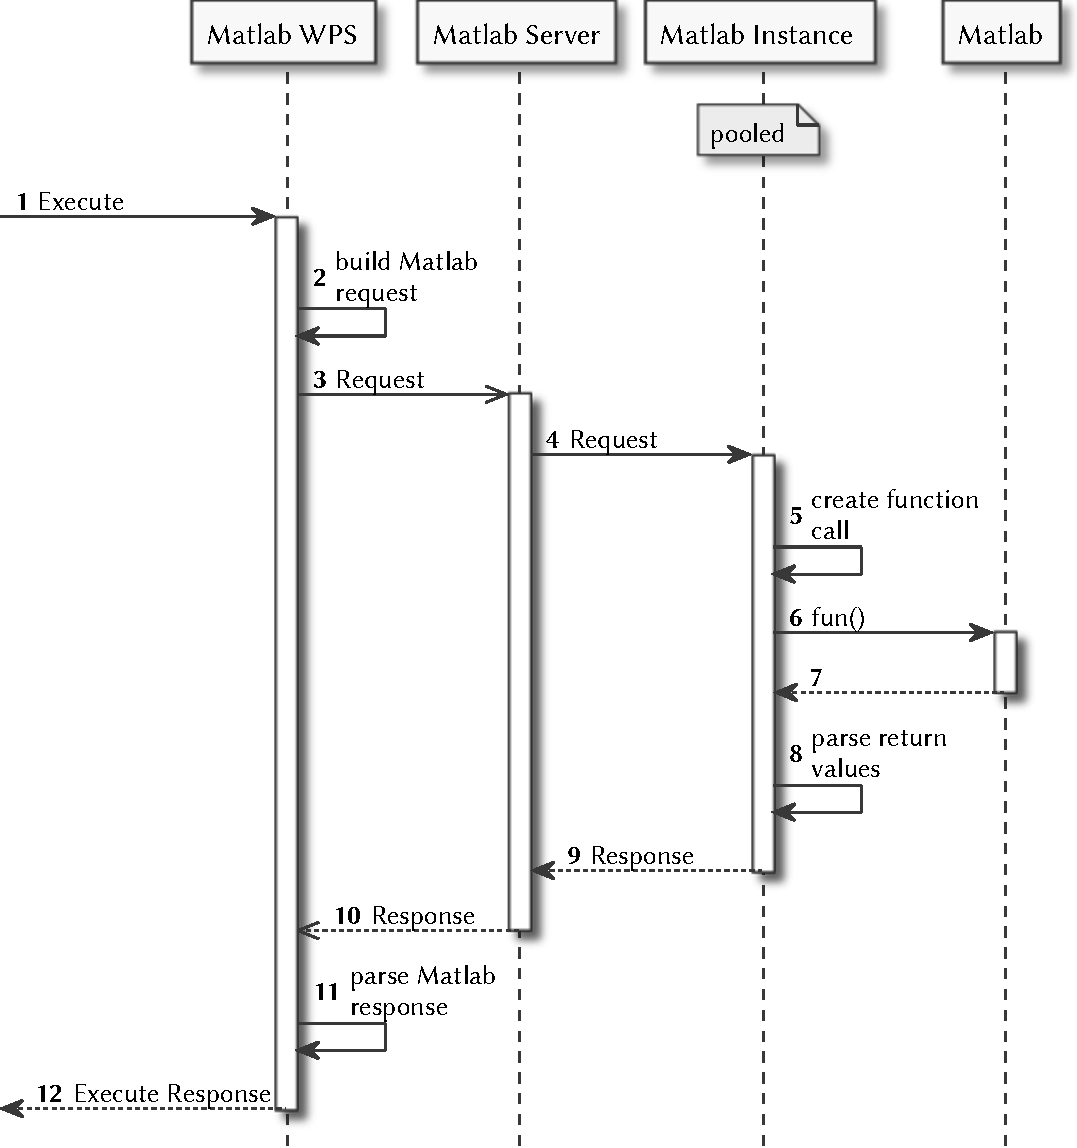
\includegraphics[width=.8\textwidth]{figures/sequence-diagramm-mwps.pdf}
		\caption{\label{fig:sd:mwps} Sequence diagram of the Matlab WPS.} %182x194
	\end{figure}
	\subsection{Lake-Analyzer WPS}
\section{Streaming WPS}
	\subsection{Input Types}
	\subsection{Dependencies}
	\begin{figure}[!htb]
		\centering
		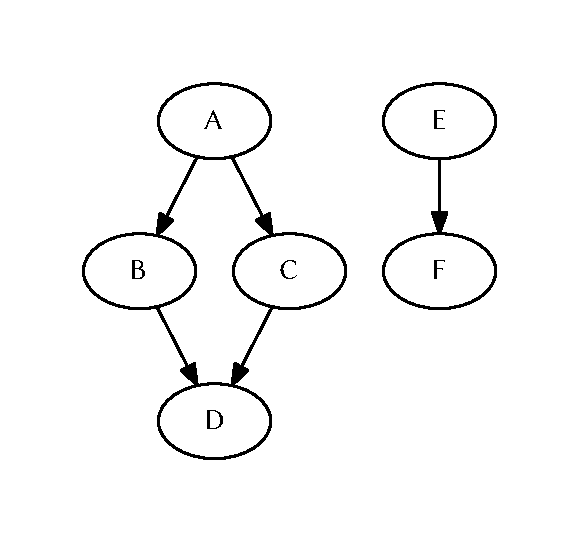
\includegraphics[width=.4474\textwidth]{figures/unordered-graph.pdf} % 98x92
		\caption{\label{fig:graph:unordered} Example for a dependency graph.}
	\end{figure}
	\begin{figure}[!htb]
		\centering
		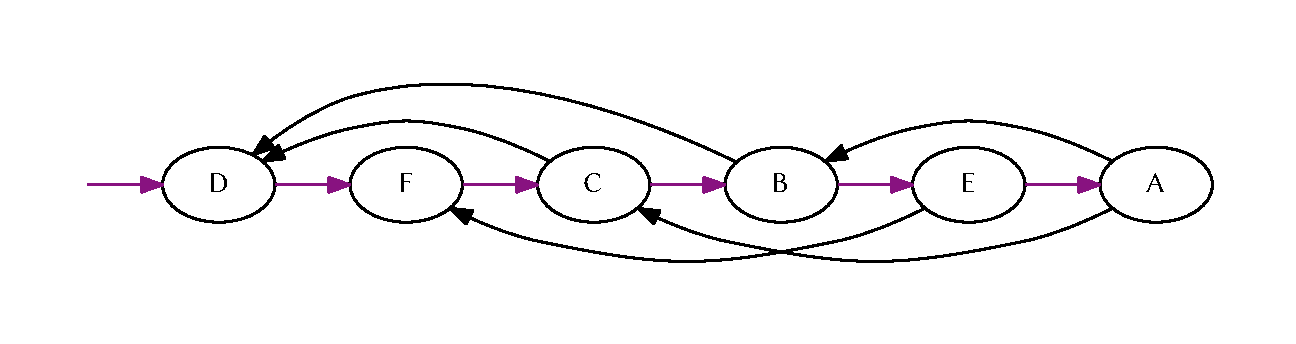
\includegraphics[width=1\textwidth]{figures/ordered-graph.pdf} % 219x58
		\caption{\label{fig:graph:ordered} Topological ordering for of the dependency graph in Figure \ref{fig:graph:unordered}.}
	\end{figure}

	\subsection{Protocoll}
	\subsection{Implementation}
	\begin{figure}[!htb]
		\centering
		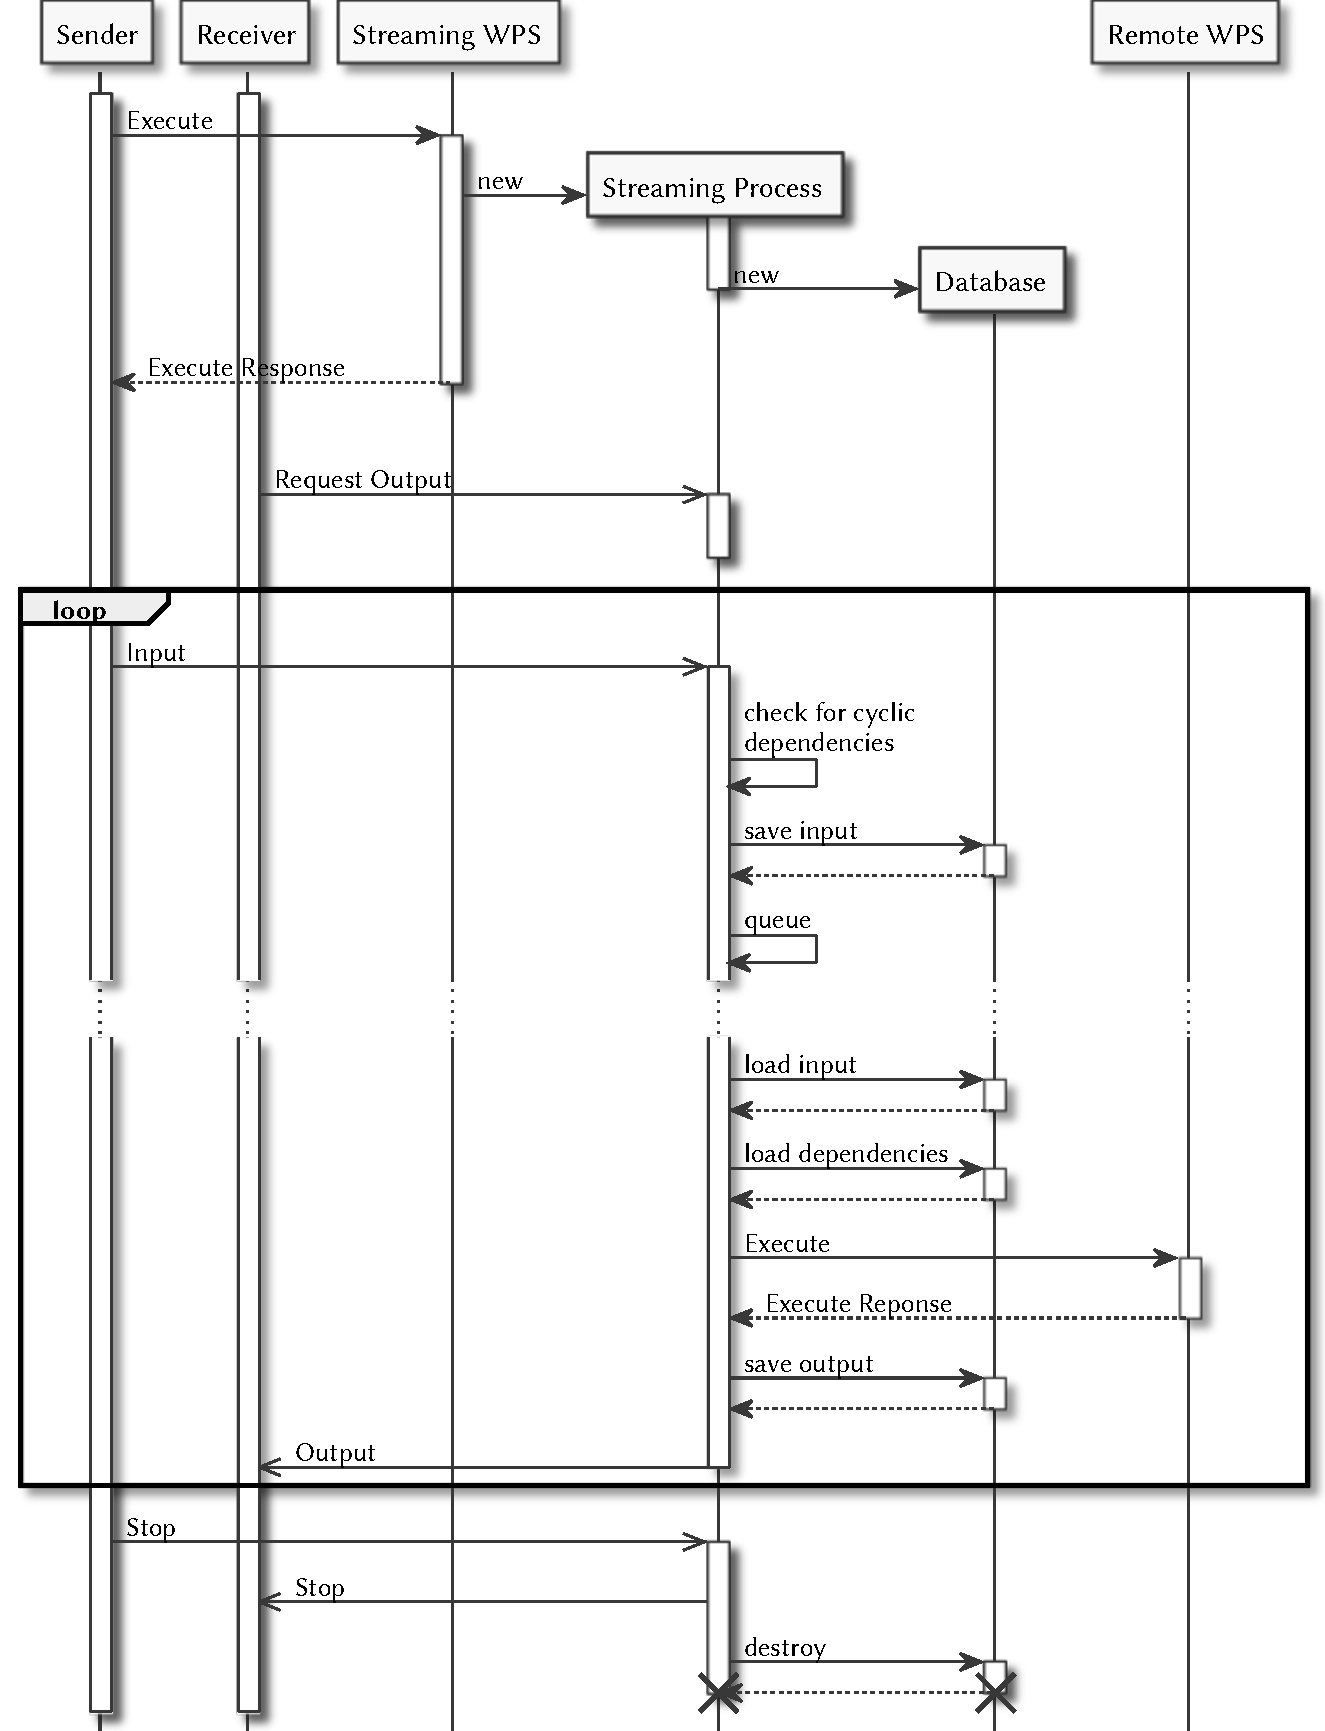
\includegraphics[width=.7868\textwidth]{figures/sequence-diagramm-swps.pdf}
		% 179x274
		\caption{\label{fig:sd:swps} Sequence diagram of the Streaming WPS.}
	\end{figure}
	\subsection{Client Implementation}
	\subsection{Streaming Lake-Analyzer WPS}
\section{Future Work}
\section{Conclusion}